% \documentclass[handout]{beamer}
\documentclass[presentation]{beamer}

\usepackage[utf8]{inputenc}
\usepackage[UKenglish]{babel}
\usepackage[T1]{fontenc}
\usepackage{lmodern}
\usepackage{booktabs}
\usepackage{caption}
\usepackage{subcaption}
\usepackage{graphicx}
\usepackage{amsmath}
\usepackage{amsfonts}
\usepackage{amssymb}
\usepackage{epstopdf}
\usepackage{hyperref}

\usepackage{tikz}
\usetikzlibrary{positioning,calc}
%\usetikzlibrary{external}
%\tikzexternalize[prefix=fig/]

% complying UK date format, i.e. 1 January 2001
\usepackage{datetime}
\let\dateUKenglish\relax
\newdateformat{dateUKenglish}{\THEDAY~\monthname[\THEMONTH] \THEYEAR}

\usecolortheme{Imperial}
% -----------------------------------------------------------------------------
%Information to be included in the title page:
\title{Addressing Security in Control Systems}
\subtitle{Overview and Current Directions}
\author{Angelo Barboni}

\date{17 September 2019}

\begin{document}
 
\begin{frame}[noframenumbering,plain]
\titlepage
\end{frame}

\begin{frame}[noframenumbering,plain]{Outline}
    \tableofcontents
\end{frame}


\section{Introduction}

\begin{frame}
	\frametitle{Security goals}

	Security (of information) can be attained if these properties are satisfied:
	\vfill
	\begin{description}
		\item[Confidentiality] Concealment or protection of sensitive information
		\item[Integrity] Trustworthiness and authenticity of data or resources 
		\item[Availability] Reliable and timely access to desired information 
	\end{description}
	\vfill
	\null
\end{frame}

\begin{frame}
	\frametitle{Motivation}
	\begin{center}
		Cyber-Physical Systems (CPS) $=$ \\ (complex, connected) software $+$ hardware
	\end{center}
	\vspace{-1ex}
	\begin{columns}
		\begin{column}{0.35\textwidth}
			Software is vulnerable: it \emph{will} be exploited. 

			\vspace{3ex}
			Security has be thought of in a system way.
		\end{column}
		\begin{column}{0.64\textwidth}
			\begin{figure}
				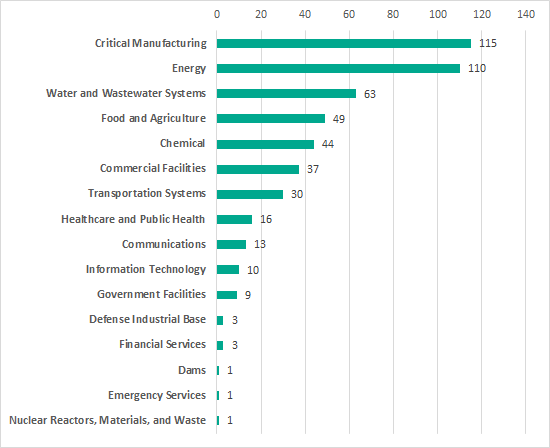
\includegraphics[scale=0.44]{fig/vuln-report-ics-cert.png}
				\caption*{\scriptsize Vulnerabilities in 2018 by sector [\href{https://ics-cert.us-cert.gov/}{\color{blue}{\underline{US ICS-CERT}}}]}
			\end{figure}
		\end{column}
	\end{columns}
\end{frame}

\begin{frame}
	\frametitle{A (possibly incomplete) series of unfortunate events}
	\setbeamertemplate{description item}[align left]
	\begin{description}
		\item[2000] Maroochy Shire incident (Australia)
		\item[2007] Aurora generator test (USA)
		\item[2009-2010] Stuxnet worm (Iran)
		\item[2014] Steel mill (Germany)
		\item[2015] Blackout (Ukraine)
		\item[2017] TRITON malware, oil spill (Saudi Arabia)
		\item[2019] Power grid DoS (USA)  
	\end{description}
\end{frame}

\begin{frame}
	\frametitle{Disclaimer}

	The topic of security encompasses many fields, from dedicated software security (PLCs, SCADA systems), to application specific cases (power networks, mobile networks, multiagent systems, etc.).

	\vfill
	We follow a generic system (model-based) approach.
\end{frame}

\AtBeginSection[]
{
  \begin{frame}[noframenumbering,plain]{Outline}
    \tableofcontents[currentsection,hideallsubsections]
  \end{frame}
}

\section{Modelling}

\begin{frame}
	\frametitle{System model}
	We consider dynamical systems in the form 

	\begin{align*}
		%\label{eq:dynsys}
		\mathcal P: \left\lbrace
		\begin{aligned}
			&\dot x = f(t,x,\textcolor{red}{\tilde u},w) \\
			&y = h(t,x,\textcolor{red}{\tilde u},v),
		\end{aligned}\right.
	\end{align*}

	but typically linearity is assumed 

	\begin{align*}
	%\label{eq:ltiplant}
	\mathcal P : \left\lbrace
	\begin{aligned}
		&\dot x = Ax + B\textcolor{red}{\tilde u} + Ww\\
		&y = Cx + D\textcolor{red}{\tilde u} + Vv
	\end{aligned}\right.
	\end{align*}
\end{frame}

\begin{frame}
	\frametitle{Adversarial model}
	An attack can be described as a triplet $\{\mathcal K, \mathcal R, g\}$ of
	\smallskip
	\begin{itemize}
		\item<1-> Knowledge $\mathcal K$ on the system, i.e. system matrices, type of detector used, etc.
		\item<2-> Resources $\mathcal R$, i.e. the measurement and actuation signals that can be accessed and/or altered
		\item<3> Attack strategy $g$ that describes the (unknown) attack strategy as some function of the available information.
	\end{itemize}	
\end{frame}

\begin{frame}
	\frametitle{Adversarial model (cont'd)}
	\begin{columns}
		\begin{column}{0.49\textwidth}
			\resizebox{\textwidth}{!}{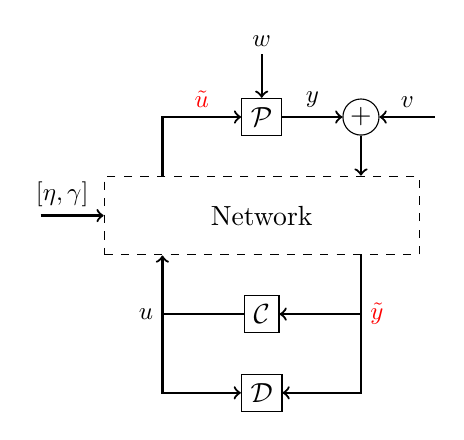
\begin{tikzpicture}{node distance=.5cm,semithick}

\node[draw] (plant) at (0,0) {$\mathcal{P}$};
\node[
   draw,
   dashed,
   minimum width = 4cm,
   minimum height = 1cm,
   below = .5cm of plant 
] (network) {Network};
\node[draw, below = .5cm of network] (controller) {$\mathcal{C}$}; 
\node[draw, below of = controller] (detector) {$\mathcal{D}$};

\node[draw, circle, inner sep = 1pt] (outnode) at ($(plant.east)+(1,0)$) {$+$};
\coordinate (innode) at ($(plant.west)+(-1,0)$);

% Connecting Arrows
\begin{scope}[every node/.style={scale=.9}]
\draw [thick,->] (plant) edge node [above] {$y$} (outnode) 
                 (outnode) edge (network.north -| outnode);
\draw [thick,->] (network.south -| outnode) |- node [right] {$\color{red}{\tilde y}$} (controller.east);
\draw [thick,->] (network.south -| outnode) |- (detector.east);
\draw [thick,->] (2.2,0) -- node [above] {$v$} (outnode.east);
\draw [thick,->] (controller.west -| innode) |- (detector.west);
\draw [thick,->] (controller.west) -| node [left] {$u$} (network.south -| innode);
\draw [thick,->] (network.north -| innode) |- (innode) -- node [above] {$\color{red}{\tilde u}$} (plant.west);
\draw [thick,->] ($(network.west) + (-0.8,0)$) -- node [above, xshift=-4pt] {$[\eta, \gamma]$} (network.west);
\draw [thick,->] (0,0.8) -- node [above, yshift=8pt] {$w$} (plant.north);
\end{scope}

\end{tikzpicture}}
		\end{column}
		\begin{column}{0.5\textwidth}
			An attacker may record
			\begin{align*}
				\left\lbrace
				\begin{aligned}
					&\nu = \textcolor{red}{\Upsilon_u} u \\
					&\xi = \textcolor{red}{\Upsilon_y} y
				\end{aligned}\right.
			\end{align*}
			\pause 
			... or inject signals $\eta$ and $\gamma$:
			\begin{align*}
				\left\lbrace
				\begin{aligned}
					&\tilde u = u + \color{red}{\eta} \\
					&\tilde y = y + \color{red}{\gamma}
				\end{aligned}\right.
			\end{align*}
		\end{column}
	\end{columns}
\end{frame}

\begin{frame}
	\frametitle{Detector model}
	We consider a residual generator as
	\begin{align*}
		\mathcal D: \left\lbrace
		\begin{aligned}
			&\dot s = A_d s + B_d u + K_d \color{red}\tilde y \\
			&r = C_d s + D_d u + E_d \textcolor{red}{\tilde y} 
		\end{aligned}\right. 
	\end{align*}
	with a threshold $\theta : r < \theta$ when there is no attack, and vice versa under attack.\\[1ex]
	If the distribution of $r$ is known, statistical tests can be used.
\end{frame}

\begin{frame}
	\frametitle{Section remarks}
	\begin{itemize}
		\setlength{\itemsep}{2ex}
		\item<1-> This framework is similar to the FDI case, however attacks are different in that:
		\begin{itemize}
			\item Strategy $g$ is not bound by the fault's physics
			\item $g$ can be designed with the \emph{purpose} of impacting the system \emph{and} satisfy $\theta$
			\item Multiple attackers can cooperate
		\end{itemize}

		\item<2-> This choice of dynamical system is not unique, and restrictive in fact. 
		Discrete-event and hybrid systems are also valid, yet more complicated.
		Same goes for distributed systems.
	
		\item<3> The detector is model-based. What about data-driven methods? And temporal logics? 
	\end{itemize}
\end{frame}

\section{Taxonomy}

\begin{frame}
	\frametitle{A CIA-based classification}

	We can divide attacks in
	\smallskip
	\begin{itemize}
		\setlength{\itemsep}{2ex}
		\item Disclosure attacks
		\item Integrity attacks
		\begin{itemize}
			\item False-data injections
			\item Zero-dynamic attacks
			\item Replay attacks
			\item Covert attacks
		\end{itemize}
		\item Denial of Service (DoS) attacks
	\end{itemize}	
\end{frame}

\section{Distributed Systems}

\section{What's next?}

 
\end{document}